\documentclass[11pt]{article}
\usepackage[margin=1.1in]{geometry}
\usepackage{amsmath,amssymb,amsthm}
\usepackage{booktabs}
\usepackage{array}
\usepackage{tabularx}
\usepackage[protrusion=true,expansion=false]{microtype}
\usepackage[table]{xcolor}
\usepackage{enumitem}
\usepackage{titlesec}
\usepackage{tikz}
\usepackage{float}
\usetikzlibrary{arrows.meta,positioning,fit,calc}
\usepackage{hyperref}

\hypersetup{colorlinks=true, linkcolor=blue!60!black, urlcolor=blue!60!black, citecolor=blue!60!black}
\usepackage[skip=0.6\baselineskip, indent=0pt]{parskip}

\titleformat{\section}{\large\bfseries}{\thesection.}{0.7em}{}
\titleformat{\subsection}{\normalsize\bfseries}{\thesubsection.}{0.6em}{}

\newcommand{\vmax}{V_{\max}}
\newcommand{\Tc}{T_{\mathrm{close}}}
\newcommand{\tx}[1]{\texttt{#1}}
\newcolumntype{L}{>{\raggedright\arraybackslash}X}

\renewcommand{\arraystretch}{1.3}
\rowcolors{1}{}{black!5}

\definecolor{coop}{RGB}{232,245,233}
\definecolor{chainc}{RGB}{255,228,225}
\definecolor{proofc}{RGB}{230,240,255}
\definecolor{hubc}{RGB}{255,243,214}

\title{\textbf{Lichen over BitVMX}\\the dispute, as built and measured}
\author{waxwing}
\date{Version 0.1, October 2026\\[2pt]\small a companion to \emph{Lichen}, version 0.2~\cite{lichen}}

\begin{document}
\maketitle

\begin{abstract}
Lichen~\cite{lichen} lets a user withdraw a hub's layer-2 tokens as
bitcoin from a two-party contract with the hub, and settles a refused
withdrawal on Bitcoin by checking a Groth16 proof of the withdrawal
statement. The main paper treats the on-chain check as a gadget with a
narrow interface. This paper describes the gadget that is built: BitVMX's
interactive search~\cite{bitvmx} over the execution of a fixed RISC-V
program, the Groth16 verifier, played as a chain of pre-signed
transactions between the user and the hub. We give the transaction graph
leaf by leaf, the windows, the fees and the payout, and the costs
measured on regtest and on Mutinynet with the current statement: a false
claim disproved is 100~kvB in 23 transactions, a lie about a memory read
200~kvB in 25, an exit against a vanished hub 23~kvB in 5, and a
contract pre-signs 141 transactions. From those figures we derive the
reserves a contract needs and the number of contracts a hub can hold
before congesting the chain becomes a profitable attack.
\end{abstract}

\tableofcontents

\section{Scope}
\label{sec:scope}

The main paper~\cite{lichen} describes the contract between a user,
Alice, and a hub; the layer 2 and its withdrawal statement; anchoring and
finality; and the economics of reserves and mass exit, all in terms that
do not depend on how a disputed proof is checked on Bitcoin. It asks of
the on-chain gadget only this:
\begin{quote}
given a proof whose public input binds the program and its journal
$b \,\|\, c \,\|\, D$, adjudicate a two-party claim on Bitcoin: the
contract's fixed terms ($c$, $D$, the program) checked, $b$ readable by
Script for a variable payout, the loser paying.
\end{quote}
and summarises any gadget by a handful of numbers: the bytes and
transactions of an exit against an absent hub and of a dispute played
to the end, each side's heaviest move within one window, the dispute's
duration, the pre-signed set and the setup per contract.

This paper fills in those numbers for BitVMX, as built in the proof of
concept~\cite{lichencode,lngapcode}, and explains where they come from.
Everything upstream of the Groth16 proof (the guests, RISC Zero's STARKs
and recursion, the wrap) is unchanged by the choice of gadget and is
covered in the main paper and the pipeline note~\cite{pipeline}; we
start where the proof becomes a claim about a program run.
Table~\ref{tab:summary} collects the results.

\begin{table}[!htp]
\centering
\small
\begin{tabularx}{\linewidth}{>{\raggedright\arraybackslash}p{62mm}L}
\toprule
parameter & BitVMX, as built \\
\midrule
exit against a vanished hub & 23.1~kvB, 5 transactions (Mutinynet) \\
a true claim refused and played to the end & about 120~kvB, 23 transactions (the sum of measured parts; 122.9~kvB measured on regtest with the older 43-word input) \\
a false claim disproved & 100.4~kvB, 23 transactions (Mutinynet) \\
the worst case: a lie about a read, disproved & 200.5~kvB, 25 transactions at 66 hops (Mutinynet); about 212~kvB at the 86-hop maximum (est.) \\
Alice's heaviest move due within one window & her proof of the last step, 25.2~kvB \\
the hub's heaviest move due within one window & its path, \tx{combine\_8}, about 93~kvB (81.1~kvB measured at 7 chunks) \\
times Alice must act in a full dispute & 13 \\
duration against a staller & about $10\,w_H + w_P$ blocks (hostile hub), $11\,w_A$ (hostile user) \\
pre-signed per contract & 141 transactions, 169 inputs \\
the links' fee floors (the reserve's floor) & 197,356~sats \\
setup beyond pre-signing & none: no garbling, no trusted setup of its own \\
\bottomrule
\end{tabularx}
\caption{The gadget's parameters, for the main paper's model. Sizes are
virtual bytes as mined, including fee inputs where a transaction takes
one; Section~\ref{sec:costs} gives the parts and their sources.}
\label{tab:summary}
\end{table}

\section{The disputed program}
\label{sec:program}

\subsection{One program for every withdrawal}

Alice's withdrawal proof is a Groth16 proof (BN254) that RISC Zero's
recursion verified a succinct receipt of the withdrawal guest, with
journal $b \,\|\, c \,\|\, D$~\cite{pipeline}. The claim taken to Bitcoin
is about the run of a fixed program on that proof:
\begin{quote}
FairgateLabs' Groth16 verifier for BitVMX~\cite{bitvmxcpu}, compiled to
RISC-V, run on Alice's 204-byte input, halts with exit code~0.
\end{quote}
The verifier's ELF is FairgateLabs' as shipped, pinned by its SHA-256
(\texttt{2b96e192\ldots}); the emulator and the scripts are BitVMX-CPU
with two bug fixes and the authenticated jump list of
Section~\ref{sec:reads} added, in a fork~\cite{bitvmxfork}. The verifier
has RISC Zero's verifying key, control root and BN254 control id
compiled in, so it accepts exactly the receipts of RISC Zero's 3.0
release family. It decompresses the proof's three points, recomputes
RISC Zero's claim digest from the image id and the journal, combines the
verifying key's points by the public inputs and checks the pairing
equation, halting with 0 if it holds. That takes about 478 million
RISC-V steps (477,943,091 on a reference input; the count varies by some
hundreds of thousands with the input), about a minute in BitVMX's
emulator on a laptop, two with the trace hashed.

\subsection{The input words}

The input is 51 four-byte words. Alice signs each with its own one-time
key (Section~\ref{sec:wots}) when she takes her claim on chain, so the
contract can read some of them and check others against its terms:
\begin{center}
\small
\begin{tabular}{llll}
\toprule
words & content & published in & used by the contract \\
\midrule
0 & the journal's length in words (10) & \tx{escalate} & checked (\tx{journal\_len}) \\
1--8 & the withdrawal guest's image id & \tx{escalate} & checked (\tx{image\_1}--\tx{image\_8}) \\
9--40 & the proof's three points, compressed & \tx{inputs} & by the search only \\
41 & $b$ & \tx{escalate} & read by the payout \\
42 & $c$, the contract's memo & \tx{escalate} & checked (\tx{memo}) \\
43--50 & $D$, the contract's identifier & \tx{inputs} & checked (\tx{deployment\_1}--\tx{deployment\_8}) \\
\bottomrule
\end{tabular}
\end{center}
Each check is a leaf of the dispute's first output, spendable by the hub
alone and at once: it re-verifies Alice's signature on the word and
succeeds if the signed value differs from the contract's, taking the
whole contract. So a proof of another program (the image id), for
another contract (the memo) or against another deployment, history or
finality threshold ($D$) loses before any search. The image-id check is
essential: the verifier would accept a valid proof of \emph{any}
program. One image id suffices because the withdrawal guest has the
chain guest's image id built in. Words are split between two
transactions only because of Script's stack (Section~\ref{sec:escalate}).

\section{Building blocks}
\label{sec:blocks}

\subsection{Values Script can read: Winternitz signatures}
\label{sec:wots}

Script checks signatures only over the spending transaction, never over
a message of the signer's choosing, so a value chosen during a dispute
(an input word, a hash of the trace, a choice) is carried by a
Winternitz one-time signature, which Script verifies by hashing alone
and which leaves the signed digits on the stack for the rule that reads
them~\cite{bitvm,bitvmx}. Digits are base 16: a key for $n$ bytes signs
$2n$ message digits and a checksum, so a four-byte word has 10 digits, a
20-byte hash 43, a one-byte choice 4. Each digit costs two witness items,
a 20-byte chain value and the digit. Keys are derived from each party's
seed per contract, exchanged when the contract opens, and used once:
signing two values under one key is \emph{equivocation}, which a leaf
can prove by showing both signatures, giving the output to the other
side.

Script's stack holds at most 1,000 items, the witness counted, so a
single input can carry, and a single rule can re-read, only a few
hundred signed bytes. Every rule therefore re-reveals only the fields it
reads; a move is split into one key per field; and large posts (the
input words, the hub's path) are split across transactions or inputs.

\subsection{Pre-signed chains}

Every step of the dispute is a 2-of-2 transaction between Alice and the
hub, signed by both when the contract opens. The values a step carries
travel in its witness, which its transaction id does not cover, so every
step's id is fixed in advance and the next step can be signed against
it. Pre-signing binds a transaction to the outputs it spends, so a
pre-signed chain can be shared only by paths that reach it through the
same transaction; here there is one, \tx{escalate}, and the whole
dispute is pre-signed once, linear in the search's length. What cannot
be pre-signed is a spend whose outputs depend on the moment (a
disprove, a check, a verdict, a sweep): these are \emph{runtime} spends
of leaves that need only the spender's key and its proof of a lie, and
they pay the spender's own wallet.

\subsection{BitVMX's search}
\label{sec:search}

BitVMX~\cite{bitvmx} settles a claim about a RISC-V program's run. The
prover (Alice) claims that the program, on her signed input, halts after
$n$ steps; each step's effect is hashed into a chain $h(1), h(2),
\ldots$, and she commits to the last hash. If the verifier (the hub)
disagrees, they search. In each round the prover posts the hashes at
$k-1$ evenly spaced steps of the interval in dispute, and the verifier
names the segment where it first disagrees. With $k = 8$ and at most
$2^{29}$ steps, ten rounds suffice: rounds 1--9 post seven hashes and
choose among eight segments (3 bits each), round 10 posts three and
chooses among four (2 bits), and the hub's ten choices, concatenated,
are the step $t$ they agree on, with disagreement on $h(t+1)$. The
prover then posts her record of step $t+1$: the instruction, the values
it read (and the step that last wrote each), what it wrote, and the
hashes on either side. Either her record proves, by BitVMX's verification
script for its class of instruction, that step $t$'s hash leads to step
$t+1$'s, or the record disagrees with the program, its input or the
search, and the hub disproves it.

\subsection{Reads and the authenticated jump list}
\label{sec:reads}

A step's hash covers what the step writes, not what it reads; a read's
value is whatever was last written to its address. So Alice could claim
a false value for a read, naming a plausible step as its last write,
and execute the instruction faithfully on it: her chain would diverge
there, the search would find the step, and her proof of it would pass.
BitVMX catches this with a second search for the read's last write, as
long again as the first. Here the trace is hashed instead as an
\emph{authenticated jump list}, after S.~D.~Lerner~\cite{bitvmxinnov}:
\[
  h(i) = \mathrm{BLAKE3}\big(h(i-1) \,\|\, h(\mathit{jump}(i)) \,\|\,
  \mathit{write}_i \,\|\, i\big)_{[0,20)},
\]
where $\mathit{jump}(i)$ is an earlier step fixed by the number $i$
alone, so that any step reaches any earlier one in at most 86 hops (about
52 on average at $2^{29}$ steps), each to the previous step or to the
long jump. A genuine hash commits to its step number, so its back-links
are the genuine hashes of the steps it names. To show a false read, the
hub posts the hashes along a path from the agreed $h(t)$ back to the
last write, and the write's preimage; its verdict wins if the write
contradicts Alice's read (another value at the step she names, or a
later write to her address). Alice, holding the true history, may
challenge any hop she finds false, and the hub must then reveal that
step's preimage, which must hash to the posted hash and link to the
next, so a forged path loses at its first false hop. The same path
settles a second lie the jump list makes possible: Alice's record
commits to the hash of her step's long jump, and a false one would let
a valid write prove on a false chain; the hub's path to
$\mathit{jump}(t+1)$ shows the true hash. Where BitVMX needs a second
search, this needs three or four more transactions
(Section~\ref{sec:tail}).

\section{The transaction graph}
\label{sec:graph}

Figure~\ref{fig:graph} shows the graph. Its outputs are \emph{carried}
values: each link of the chain moves the whole contract, less a fee
floor (Section~\ref{sec:fees}), into the next output, so whichever leaf
finally spends an output settles the whole contract.

\begin{figure}[!htp]
\centering
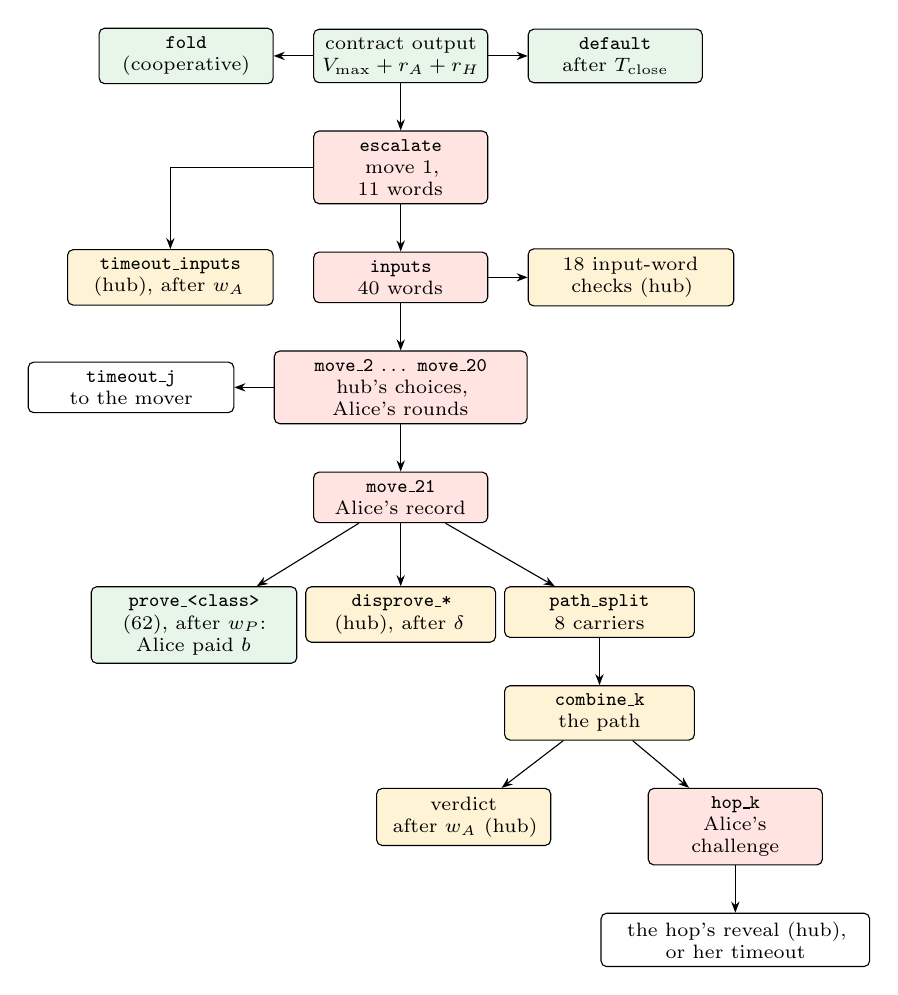
\begin{tikzpicture}[
  font=\scriptsize,
  tx/.style={draw, rounded corners=2pt, align=center, inner sep=3pt, text width=#1},
  tx/.default=20mm,
  >={Stealth[length=4pt]},
  node distance=6mm and 5mm,
]
\node[tx, fill=coop] (c) {contract output\\$\vmax + r_A + r_H$};
\node[tx, fill=coop, left=of c] (fold) {\tx{fold}\\(cooperative)};
\node[tx, fill=coop, right=of c] (def) {\tx{default}\\after $\Tc$};
\node[tx, fill=chainc, below=of c] (esc) {\tx{escalate}\\move 1, 11 words};
\node[tx, fill=chainc, below=of esc] (inp) {\tx{inputs}\\40 words};
\node[tx, fill=hubc, right=of inp, text width=24mm] (chk) {18 input-word\\checks (hub)};
\node[tx, fill=hubc, left=of inp, text width=24mm] (tin) {\tx{timeout\_inputs}\\(hub), after $w_A$};
\node[tx, fill=chainc, below=of inp, text width=30mm] (mv) {\tx{move\_2} \ldots\ \tx{move\_20}\\hub's choices, Alice's rounds};
\node[tx, left=of mv, text width=24mm] (tj) {\tx{timeout\_j}\\to the mover};
\node[tx, fill=chainc, below=of mv] (rec) {\tx{move\_21}\\Alice's record};
\node[tx, fill=coop, below left=8mm and 2mm of rec, text width=24mm] (prove) {\tx{prove\_<class>}\\(62), after $w_P$:\\Alice paid $b$};
\node[tx, fill=hubc, below=8mm of rec, text width=22mm] (dis) {\tx{disprove\_*}\\(hub), after $\delta$};
\node[tx, fill=hubc, below right=8mm and 2mm of rec, text width=22mm] (split) {\tx{path\_split}\\8 carriers};
\node[tx, fill=hubc, below=of split, text width=22mm] (comb) {\tx{combine\_k}\\the path};
\node[tx, fill=hubc, below left=6mm and -6mm of comb, text width=20mm] (ver) {verdict\\after $w_A$ (hub)};
\node[tx, fill=chainc, below right=6mm and -6mm of comb, text width=20mm] (hop) {\tx{hop\_k}\\Alice's challenge};
\node[tx, below=of hop, text width=32mm] (rev) {the hop's reveal (hub),\\or her timeout};
\draw[->] (c) -- (fold);
\draw[->] (c) -- (def);
\draw[->] (c) -- (esc);
\draw[->] (esc) -- (inp);
\draw[->] (esc.west) -| (tin.north);
\draw[->] (inp) -- (chk);
\draw[->] (inp) -- (mv);
\draw[->] (mv) -- (tj);
\draw[->] (mv) -- (rec);
\draw[->] (rec) -- (prove);
\draw[->] (rec) -- (dis);
\draw[->] (rec) -- (split);
\draw[->] (split) -- (comb);
\draw[->] (comb) -- (ver);
\draw[->] (comb) -- (hop);
\draw[->] (hop) -- (rev);
\end{tikzpicture}
\caption{The dispute's graph, simplified. Red: Alice's links and the
chain of moves; yellow: the hub's moves and spends; green: settlements.
The links are pre-signed. Every link's output also has a pre-signed
timeout against the party due to move, and equivocation leaves for every
one-time key used so far.}
\label{fig:graph}
\end{figure}

\subsection{The contract output}
\label{sec:output}

The contract output holds $\vmax + r_A + r_H$ and funds no fees. Every
taproot tree in the graph has an unspendable (NUMS) internal key, so
every spend is a script path; leaves are placed by a Huffman tree of
equal weights. The contract output has three leaves:
\begin{itemize}[leftmargin=1.5em]
\item \tx{fold}: the 2-of-2, signed when the fold is agreed, not in
  advance; Alice receives $b + r_A$, the hub the rest less a fixed fee.
  (A MuSig2 key path would make this about 140~vB instead of 193.)
\item \tx{default}: after $\Tc$ (\texttt{CLTV}), pre-signed, returning
  $r_A$ to Alice and the rest to the hub.
\item \tx{escalate}: after the contract's \texttt{to\_self\_delay}
  (\texttt{CSV}), the 2-of-2 and Alice's signatures on move~1 and on
  her claim words.
\end{itemize}
The proof of concept builds contracts as standalone outputs; the same
three leaves sit in a channel commitment beside the revocation leaf
in LN-GAP's channel code~\cite{lngapcode}, where every channel update
re-signs the set for both commitments.

\subsection{The escalation and the inputs}
\label{sec:escalate}

\tx{escalate} spends the contract into the \emph{claimed output}. Its
witness carries move~1 (the claim, 28 bytes: the last step and its
hash; and round 1's seven hashes) and 11 claim words: the journal's
length, the image id, $b$ and the memo. That is 944 stack items, close
to the limit, so the other 40 words (the proof and $D$) follow in
\tx{inputs}, which spends the claimed output into the first output of
the search. The claimed output has one more leaf, \tx{timeout\_inputs},
paying the hub if \tx{inputs} has not come within Alice's window $w_A$:
the hub must have her whole input before it can run the verifier and
move.

The search's first output carries the 18 input-word checks of
Section~\ref{sec:program}, besides the leaves every output has. The hub
reads the words from both links and checks them before it moves; a
wallet refuses to escalate a claim that fails one.

\subsection{The search}
\label{sec:ladder}

After \tx{inputs}, the search alternates the hub's choices (moves 2, 4,
\ldots, 20) and Alice's rounds of hashes (3, 5, \ldots, 19), ending with
her record (move 21). Move $j$ is the link \tx{move\_$j$}, spending
output $j-1$ into output $j$; each link has two outputs, the carried
value and an \emph{anchor} for its poster's fees. Every output $j < 21$
has:
\begin{itemize}[leftmargin=1.5em]
\item \tx{post}: \texttt{1 CSV}, the 2-of-2 and the next mover's
  signatures on its move's fields: the pre-signed \tx{move\_$j{+}1$};
\item \tx{timeout\_$j$}: the 2-of-2 after the next mover's window,
  pre-signed, paying the contract to the mover of $j$, since its
  opponent failed to answer;
\item the opponent's rules on move $j$, as runtime \tx{disprove} leaves
  after a delay $\delta$: for a choice, that it is out of range;
\item \tx{equiv\_d}: one leaf for each field of each move so far, by
  which the other side shows two signatures under one key and takes the
  output (Section~\ref{sec:offchain}).
\end{itemize}
A round of Alice's is seven 20-byte hashes, 301 signed digits and 606
witness items: about 7.5~kvB. A choice of the hub's is one byte, about
0.34~kvB. The \texttt{1 CSV} on \tx{post} means the opponent's answer
can only follow a link's confirmation, so nothing but the poster's own
fee child can spend an unconfirmed link (Section~\ref{sec:fees}).

\paragraph{Windows by obligation.} A move's size, not its mover, decides
how long it may need to get into a block when blocks are full
(Section~\ref{sec:exit}), so the windows are set by what is owed: Alice
has $w_A$ for each of her moves and for \tx{inputs}; the hub has $w_H$
for each choice, a few hundred bytes; and $w_P$ for its heavy moves at
the end, the path and the disproves' opportunity before Alice may prove.
The hub offers its windows with each contract; a wallet refuses a $w_A$
shorter than the network's minimum. As configured:
\begin{center}
\small
\begin{tabular}{lrrrr}
\toprule
network & $w_A$ & $w_H$ & $w_P$ & $\delta$ \\
\midrule
regtest & 14 & 10 & 16 & 6 \\
Mutinynet (30-second blocks) & 80 & 20 & 80 & 40 \\
signet & 12 & 6 & 12 & 6 \\
testnet4 & 72 & 18 & 72 & 36 \\
\bottomrule
\end{tabular}
\end{center}
Alice's window and the path's must exceed $\delta$, so that every
runtime disprove opens before the timeout it races.

\subsection{The last step}
\label{sec:final}

Alice's final move signs five fields: her 64-byte record of step
$t+1$; $h(t)$ and $h(t+1)$; $J$, the hash of the step's long jump; and
$t+1$ itself. The record holds the step's two reads (address, value and
the step that last wrote each), its program counter and opcode, its
write (address, value, next program counter) and the agreed step $t$.
It is about 6.8~kvB. Its output has the largest tree of the graph,
about 2,200 leaves by our count:
\begin{itemize}[leftmargin=1.5em]
\item one \tx{prove\_<class>} per class of instruction in the program,
  62 for the Groth16 verifier: after $w_P$, pre-signed, paying Alice's
  payout. Its script guards the class, runs BitVMX's verification script
  for it on the record, and checks the jump-list step hash
  $\mathrm{BLAKE3}(h(t) \,\|\, J \,\|\, \mathit{write} \,\|\, t+1) =
  h(t+1)$. It re-reveals all five fields and is Alice's heaviest move:
  25.2~kvB as mined, its fee input included.
\item the hub's runtime disproves, after $\delta$, each paying it the
  output: \tx{step} (the record's $t$ is not the hub's choices),
  \tx{initial}, \tx{halt\_hash}, \tx{halt\_exit} (the claimed last step
  is not an exit with code 0: 5.1~kvB), \tx{entry\_point},
  \tx{program\_counter}, \tx{addresses\_sections}, \tx{succ},
  \tx{future\_read\_1} and \tx{\_2}, the equivocation re-sign challenges
  for every round and index (132 leaves), \tx{uninitialized\_1} and
  \tx{\_2}, \tx{initialized\_$k$} for each data chunk, \tx{opcode\_$k$}
  for each of the program's 1,773 code chunks (the opcode at the
  record's pc), and \tx{input\_$j$} for each input word (a read of an
  input word never written must equal Alice's signed word, re-revealed
  from \tx{escalate} or \tx{inputs});
\item \tx{path}: \texttt{1 CSV} and the 2-of-2, the hub's way into the
  read and jump challenges below;
\item \tx{timeout\_21}: after $w_P + w_A$, the hub's, if Alice never
  proves;
\item the \tx{equiv\_d} leaves, 82 by the final output.
\end{itemize}
The hub decides by running BitVMX's challenge selection on the record:
a mismatch with the program or the input picks the disprove; a read it
contests, or a long-jump hash that differs from its own, picks the
path; otherwise the step proves and an honest hub stops.

\subsection{The read and jump challenges}
\label{sec:tail}

A path of up to 86 hashes, 1,720 signed bytes, does not fit one input's
stack, so it is posted in chunks, one per input of one transaction. From
the final output, the hub's \tx{path\_split} makes eight \emph{carriers},
the first holding the value and the rest dust, each with a \tx{chunk}
leaf verifying one chunk's one-time signatures; \tx{combine\_$k$} spends
the first $k$ carriers, chunk $c$ in input $c$. The first chunk holds the
hops' count, their types (a nibble each: previous step or long jump),
the path's end and 8 hashes; each other chunk holds 11. Both
transactions are pre-signed, a combine for each $k$. The path's output
then has:
\begin{itemize}[leftmargin=1.5em]
\item \tx{hop}: \texttt{1 CSV}, the 2-of-2 and Alice's one-byte choice
  of a hop to challenge: the pre-signed \tx{hop\_$k$};
\item the hub's verdicts, \tx{jump}, \tx{read\_1} and \tx{read\_2},
  after $w_A$, each with the end step's 57-byte preimage: the end is
  $\mathit{jump}(t+1)$ and its hash differs from $J$, or the end is the
  read's last write and contradicts Alice's read;
\item \tx{timeout\_combine\_$k$}: after $w_P + w_A$, Alice's, if no
  verdict comes.
\end{itemize}
After \tx{hop\_$k$}, the hub has $\delta$ to reveal the challenged
hop's preimage, which must hash to its posted hash and link to the next
by the hop's type; if it cannot, Alice's \tx{timeout\_hop\_$k$} pays her
after $w_P$. A split never combined pays Alice from the first carrier
after $w_P$. A read dispute adds three or four transactions to the
search: the split, a combine and the verdict, and Alice's challenge with
its answer if she makes one.

\subsection{Off-chain play}
\label{sec:offchain}

LN-GAP lets the parties play the search off chain by exchanging signed
moves, and lets either take it on chain by \emph{replaying} the moves
so far from the signatures it holds; the \tx{equiv\_d} leaves keep a
replay faithful, since altering one of one's own moves means signing a
second value under its key. lichen does not play off chain: an honest
hub that checks Alice's proof natively, in milliseconds, has nothing to
gain from a search it will lose, and a hub that refuses is better met on
chain at once. The leaves are built and tested in LN-GAP~\cite{lngapcode}
and cost only tree depth here. What lichen does replay is its own
state: after a restart, each side re-derives its moves, deterministic
from its seed and the chain, and checks them against the links already
mined.

\section{Outcomes and the payout}
\label{sec:payout}

A dispute decides only Alice's withdrawal: $b$ if her claim stands,
nothing if it fails; the rest of $\vmax$ goes to the hub, and the loser's
reserve to the winner.

\paragraph{When Alice wins} (a proof of the last step; any timeout
against the hub; a path split and never combined, a verdict that never
comes, a hop not revealed) the terminal transaction pays a pre-signed
\emph{payout}: one output of $2^i$~sats for each bit $i$ of a 32-bit
amount from bit 9 up to the contract's size $K$ (so $b$ is rounded down
to a multiple of 512~sats, and $\vmax = 2^K - 1$), an output for the
reserves, and the remainder to the hub. Script cannot compute an amount,
but it can read Alice's signature on word 41, so each bit output has
three leaves, as for numeric DLCs~\cite{dlcnumeric}:
\begin{center}
\small
\begin{tabular}{lll}
\toprule
leaf & spent by & condition \\
\midrule
\tx{alice\_bit\_$i$} & Alice, after $\delta$ & her signature on $b$ has bit $i$ set \\
\tx{hub\_bit\_$i$} & the hub & the same signature has bit $i$ clear \\
\tx{equiv\_b\_$i$} & the hub & two signatures on different values of $b$ \\
\bottomrule
\end{tabular}
\end{center}
Since $b$ is under a one-time key, the bits Alice can take are those of
the one value she signed, and they sum to $b$; her leaves wait $\delta$
so that an equivocation can be shown first. The reserve output holds
$r_A + r_H$ less the links' floors, with Alice's leaf after $\delta$ and
an \tx{equiv\_b} leaf of its own. A bit's spend is about 320--330~vB, and
each party sweeps its outputs in one transaction; the hub finds its own
by Alice's signature, already on chain in \tx{escalate}.

\paragraph{When the hub wins} (a check, a disprove, a verdict, a hop's
reveal, or a timeout against Alice) the hub takes the output whole, both
reserves included, as a runtime spend to its wallet, or by a pre-signed
timeout paying one output.

\paragraph{The variable payout is not BitVMX's.} Any gadget needs a way
for Script to read $b$, and the bit outputs need only the one-time
signature on it, so this section carries over unchanged to other
gadgets; the main paper describes it as part of the contract.

\section{Fees}
\label{sec:fees}

\paragraph{Links} (\tx{escalate}, \tx{inputs}, the moves, the split,
the combines, the hops) must keep their transaction ids, since the next
link was signed against them, so nothing can be added to them. Each is
an ordinary version-2 transaction that pays a \emph{floor} of 1~sat/vB
of its own out of the carried value, enough to relay alone, and carries
a 330-sat anchor that only its poster can spend; when the feerate is
higher, the poster adds a child spending the anchor and a coin of its
own. Because the opponent's next move waits a block after the link
confirms (\texttt{1 CSV}), only the poster's child can sit on an
unconfirmed link: the challenge and response happen on chain, not in the
mempool, and there is nothing for pinning to work on. So a link may be
as large as standard relay allows (100~kvB), where TRUC's rules would
cap it at 10~kvB; the escalation is 11.6~kvB and a path's combine up to
93. A floor is computed from an upper bound of its link's size, every
digit at full length and the leaf at its tree's greatest depth, so the
floors are a property of the statement, not of the keys. The deepest
dispute, a worst-case read, spends 197,356~sats of floors and anchors,
about half of it in the combine.

\paragraph{Terminals} (the timeouts, the proofs, the default) are spent
only by runtime leaves, so their ids may change. Both parties sign them
\texttt{ALL|ANYONECANPAY} at no fee, committing to their input and all
their outputs, and the broadcaster adds one coin, sized exactly, with no
change; the feerate is chosen at broadcast. Alice keeps a fee budget for
this, by default 30,000~sats where fees are low and 150,000 elsewhere,
and a wallet refuses a contract whose heaviest terminal at the minimum
feerate, \tx{prove\_<class>} at about 26,800~sats, the budget could not
pay.

\paragraph{Runtime spends} (checks, disproves, verdicts, sweeps) are
built when needed and pay what the moment requires from the value they
take.

\section{Costs}
\label{sec:costs}

\subsection{Transactions}

Table~\ref{tab:sizes} gives each transaction's size as mined. Unless
marked, figures are from the Mutinynet trials of
October 2026~\cite{lichencode} (contracts 1001--1006), with the current
51-word input, at 1~sat/vB and so without fee children.

\begin{table}[!htp]
\centering
\small
\begin{tabularx}{\linewidth}{>{\raggedright\arraybackslash}p{70mm}L}
\toprule
transaction & size \\
\midrule
\tx{fold} (cooperative close) & 193~vB \\
\tx{escalate}: move 1 and 11 words (470 digits, 944 items) & 11.6~kvB \\
\tx{inputs}: 40 words (400 digits) & 9.9~kvB \\
the hub's choice & 0.33--0.35~kvB \\
Alice's round of seven hashes; her round 10 (three) & 7.5~kvB; 3.4~kvB \\
her record (move 21) & 6.8~kvB \\
\tx{prove\_<class>}, her proof of the last step & 25.2~kvB (an upper bound of 26.2 over all classes) \\
\tx{disprove\_halt\_exit} & 5.1~kvB \\
\tx{path\_split}; \tx{combine\_$k$}; \tx{disprove\_read\_2} & 0.6~kvB; 11.6~kvB a chunk (81.1~kvB for 7, a 66-hop path); 23.6~kvB \\
a timeout, with its fee input & 0.59--0.60~kvB \\
a bit output's spend & 0.32--0.33~kvB \\
an input-word check & 0.41~kvB (regtest) \\
\bottomrule
\end{tabularx}
\caption{Sizes as mined on Mutinynet unless marked. The escalation varies
by a few bytes with its leaf's depth in the tree.}
\label{tab:sizes}
\end{table}

Whole disputes, as played:
\begin{center}
\small
\begin{tabularx}{\linewidth}{>{\raggedright\arraybackslash}p{62mm}rrL}
\toprule
case & size & txs & source \\
\midrule
the hub vanished: escalate, inputs, a split for the fee coin, the hub's timeout, the payout's sweep & 23.1~kvB & 5 & Mutinynet, contract 1001 \\
the hub returns mid-dispute and concedes on its native check & 24.0~kvB & 5 & Mutinynet, 1002 \\
a false claim (an exit-code lie), disproved by \tx{halt\_exit} & 100.4~kvB & 23 & Mutinynet, 1003 \\
a lie about a read, disproved through a 66-hop path & 200.5~kvB & 25 & Mutinynet, 1004 \\
a true claim refused and played to the end & about 120~kvB & 23 & the sum of the parts above; 122.9~kvB measured on regtest with the 43-word input, fee children included \\
\bottomrule
\end{tabularx}
\end{center}
A true claim played through is 22 links and its terminal: escalation and
inputs 21.5~kvB, Alice's rounds 63.6, the hub's choices 3.4, her record
6.8 and her proof 25.2. Exchanging the proof for the hub's
\tx{halt\_exit} gives 100.4~kvB, the false claim exactly as measured. At
the jump list's 86-hop maximum a read's combine is about 93~kvB and the
read dispute about 212~kvB.

\subsection{Time}

\begin{center}
\small
\begin{tabularx}{\linewidth}{>{\raggedright\arraybackslash}p{70mm}L}
\toprule
item & measured \\
\midrule
the withdrawal proof (STARK), the current guest & 389,020 cycles: 74~s on an Apple M4 Pro; 359~s on a 4-vCPU x86 server \\
the Groth16 wrap & 257~s on the same server (x86 only) \\
checking the proof natively & 1.5~ms; a returning hub conceded 2.4~s after it started (contract 1002) \\
the verifier, emulated & about a minute; two with the trace hashed \\
both sides' executions over a search & about 12 minutes \\
a dispute played on regtest (51 words) & a true claim proved in 730~s, a false one disproved in 545~s \\
a hostile hub played to the payout on Mutinynet, Alice's side run by a tower & the record 15 minutes after the escalation; the payout 75 minutes after the tower started (30-second blocks) \\
\bottomrule
\end{tabularx}
\end{center}
On mainnet the windows set the time. A hub that stalls on every move
stretches a dispute to about $10\,w_H + w_P$ blocks, and a block a move
besides; a user who stalls, to about $11\,w_A$, her own money waiting. A
vanished hub's users wait only the hub's first window, $w_H$, after
their input. With $w_A = 144$, $w_H = 12$ and
$w_P = 288$, a hostile hub can stretch a dispute to about 430 blocks,
three days, and a vanished hub's users wait two hours after their input.

\subsection{Pre-signing}

A contract pre-signs 141 transactions with 169 inputs: \tx{default};
\tx{escalate} and \tx{timeout\_inputs}; the 21 links from \tx{inputs}
to \tx{move\_21} and their 21 timeouts; the 62 proofs; and the tail
(\tx{path\_split} and its timeout, and for each $k$ from 1 to 8,
\tx{combine\_$k$}, \tx{hop\_$k$} and their timeouts). The hub builds the
set and signs; Alice rebuilds it herself, verifies the hub's 169
signatures and signs; the hub verifies hers before it broadcasts the
funding. A mock statement for tests needs 47.

\section{Reserves}
\label{sec:reserves}

The main paper argues that each side's reserve must at least cover the
other side's fees in a dispute it loses, and that the hub's binds,
since it must make Alice whole for a refused withdrawal however small
her balance. Here that floor is concrete. The links' floors alone,
fixed when the contract is signed, reach 197,356~sats in the deepest
dispute; lichen's hub sets $r_H$ to the larger of its share of the cap
and that figure. At a prevailing feerate $f$, what the reserve must cover
is roughly Alice's side of a dispute, about 117~kvB (escalation and
inputs 21.5, her rounds 63.6, her record 6.8, her proof 25.2), times
$f$: 117,000~sats at 1~sat/vB, 234,000 at 2, 1.2 million at 10. On top
of that the hub locks the cap's headroom $\vmax - D$, so a user holding
50,000~sats costs the hub about as much locked capital as one holding
two million; under this gadget, the contract suits balances from about
half a million sats, and comfortably from a few million.

\section{Mass exit}
\label{sec:exit}

\subsection{By bytes}

\begin{center}
\small
\begin{tabularx}{\linewidth}{>{\raggedright\arraybackslash}p{58mm}rrL}
\toprule
exit & per user & per block & per day; per month, at a quarter of each block \\
\midrule
the hub present: a fold and its sweep & 0.3~kvB & 3,400 & 120,000; 3.7M \\
the hub gone & 23.1~kvB & 43 & 1,600; 47,000 \\
the hub refuses a true claim to the end & 120~kvB & 8 & 300; 9,000 \\
the hub disproves a false claim & 100.4~kvB & 10 & 360; 10,800 \\
the hub disproves a read lie & 200--212~kvB & 5 & 170; 5,100 \\
\bottomrule
\end{tabularx}
\end{center}
A day is 144 blocks, a month 4,320, a block 1~MvB. With the hub gone,
each exit has until its contract's $\Tc$, so staggered expiries spread
the load.

\subsection{Congestion}

When one side is hostile, a different limit binds. To make an honest
party miss a move, the attacker must outbid it in every block of that
move's window of $w$ blocks. That costs about the same whether one
defender is shut out or many, so it pays only when the moves due in one
window could not all fit in it anyway: $N s > w \cdot 1\,\mathrm{MvB}$,
for $N$ contracts whose heaviest move due in a window is $s$. This is
Flood \& Loot~\cite{floodloot} in lichen's form. We take the attacker's
best case, every contract's heaviest move due in the same window:
hostile users choose when to escalate, and a hostile hub can delay each
of its replies by up to $w_H$ to bunch them.

\begin{center}
\small
\begin{tabularx}{\linewidth}{>{\raggedright\arraybackslash}p{52mm}LL}
\toprule
& a hostile hub, against honest users & hostile users (read lies), against an honest hub \\
\midrule
the defender's heaviest move in one window, $s$ & Alice's proof of the last step, 25.2~kvB & the hub's \tx{combine\_8}, about 93~kvB \\
contracts safe at $w = 12$ (two hours) & 480 & 130 \\
at $w = 144$ (a day) & 5,700 & 1,550 \\
at $w = 1{,}008$ (a week) & 40,000 & 10,800 \\
the window needed for 3,000 contracts & 76 blocks (13 hours) & 280 blocks (2 days) \\
for 60,000 & 1,510 blocks (10 days) & 5,580 blocks (39 days) \\
\bottomrule
\end{tabularx}
\end{center}
The escalation and \tx{inputs} (21.5~kvB) are not counted: they run
against $\Tc$, not a window, and only \tx{inputs} has a window, Alice's
own, opened by her own escalation. Each window holds only its own
moves, so only the two heavy ones grow with $N$: Alice's proof, due in
the $w_A$ after $w_P$, and the hub's path, in $w_P$. The hub's choices,
0.34~kvB each, keep $w_H$ short, and that is the window a vanished
hub's users wait. The second column binds: the liar picks the lie, and
a read lie maximises the hub's load in one window.

\subsection{What would improve it, within BitVMX}

\begin{itemize}[leftmargin=1.5em]
\item \emph{The path in its own windows.} Posting each chunk of the
  path as its own transaction in its own window, only in the read-lie
  tail, would bring the hub's $s$ down to its read verdict, 23.6~kvB:
  about 6,000 contracts per day-long window instead of 1,550.
\item \emph{A shorter jump list.} Lerner's tighter long-jump function,
  about $\log_2 n + 3\log_2\log_2 n$ hops (some 45 instead of 86), or a
  counter moving over a step number's set bits only, shrinks the path,
  its combine and the floors about in proportion.
\item \emph{The inputs on demand.} With the hub gone, Alice could
  escalate with only $b$ and the checked words; a present hub would
  post a small pre-signed demand, and only then would she owe the rest.
  The absent-hub exit would fall from 23~kvB to about 3--4 (est.).
\item \emph{Delegated fold signing.} Judging a fold needs only public
  layer-2 data, so a successor or backup key (even the sequencer's) could
  sign folds while the hub is down; a rogue backup can only overpay
  users, the hub's own risk. An outage then costs 0.3~kvB an exit, not
  23.
\item \emph{A chess clock.} Union~\cite{union} gives each party a budget
  for all its moves together, so a staller stretches the dispute only to
  the two budgets, not to ten windows; the price is extra pre-signed
  transactions, published only against a staller.
\end{itemize}
Smaller rounds would not help Alice's side: her heaviest move is the
proof of one step, whatever the search's arity.

\section{Alice's liveness and the tower}
\label{sec:tower}

A dispute runs for hours on Mutinynet and days on mainnet, and Alice
must answer each of the hub's choices within $w_A$. Her moves follow
from her trace, which anyone with her input can compute, but a move is
also her commitment: hashes from her trace signed with her one-time keys
for that move, and which hashes depends on the hub's earlier choices, so
the signatures cannot be made in advance. That is what makes delegation
under BitVMX harder than in Lightning, where a watchtower holds
pre-signed penalties.

\paragraph{As built.} lichen's tower runs the wallet's own dispute
engine from a \emph{package} Alice exports: the contract's record with
the whole pre-signed set; $b$, as her signature rather than its key, so
the tower cannot claim another amount; the seeds of her other input-word
keys, her move keys and her hop keys; her fee budget's key; and,
optionally, her withdrawal input and chain receipt so that it can prove
the withdrawal itself. It reads the chain through two Esplora servers
that must agree, plays the whole dispute, read challenges included, to
the payout, and stops: Alice sweeps with her wallet, which checks that
the payout is a terminal of her contract. The worst a tower can do is
make wrong moves, equivocate, stay silent or spend the fee budget, so it
is trusted like her own machine. The intended form is her own: a
container on a rented server, started when a fold is refused and
discarded after, since in a standalone contract only Alice can start a
dispute and nothing can be broadcast against her before she does. In
the Mutinynet trials such a tower, on a 4-vCPU server, proved the
withdrawal and played a hostile hub to the payout in about 75 minutes.

\paragraph{Keyless moves} would let anyone post them: Alice would sign a
Merkle root over her trace when she escalates, and each later move would
be an opening of it. The opening must be checked when posted, or a
dishonest poster could publish garbage first; without \texttt{OP\_CAT}
a 29-level path cannot be hashed natively, and emulating the hash in
Script would make each move hundreds of times larger. With
\texttt{OP\_CAT} it would be cheap.

\section{Scenarios}
\label{sec:scenarios}

\begin{center}
\small
\begin{tabularx}{\linewidth}{p{58mm}L}
\toprule
scenario & outcome under BitVMX \\
\midrule
the hub disappears & Alice escalates and posts her inputs; the hub never moves; \tx{timeout\_1} pays $b$ and both reserves \\
the hub refuses a valid claim & the search on chain; Alice proves the last step; $b$ and both reserves \\
Alice claims a return she never made & the verifier halts with failure; the hub's \tx{halt\_exit} takes everything \\
Alice props up a false claim with a false read, or a false long jump & the hub's path through its history to the read's last write (or to the long jump); unless she shows a hop false, its verdict takes everything \\
the hub forges a hash in that path & Alice challenges the hop; the hub cannot reveal it; her timeout pays $b$ and both reserves \\
the hub splits the path and never combines it & the first carrier's timeout pays $b$ and both reserves \\
Alice escalates and never posts her inputs & \tx{timeout\_inputs} pays the hub \\
Alice probes: a false claim, abandoned when the hub answers & she loses by timeout: everything, her reserve included, to the hub \\
a proof of another program, for another contract or against another history or work & an input-word check takes the contract before any search \\
Alice signs two values of $b$ & the hub takes the bit outputs and the reserves with \tx{equiv\_b} \\
either side signs two values under one move key & the other takes the output with \tx{equiv\_d} \\
either side forces the search on chain to cause trouble & the outcome is unchanged; each pays its own moves' fees beyond the floors, and the loser's reserve covers the floors \\
\bottomrule
\end{tabularx}
\end{center}

\section{Beside the bridges}
\label{sec:bridges}

BitVMX's search is also the dispute of Union~\cite{union}, a bridge to
Rootstock by BitVMX's own authors, where every pair of a committee of
functionaries pre-signs a game for every peg-in, 4-ary, about 270~kvB at
worst, with a nested game for a challenge to the claimant's chain of
headers. A lichen contract is Union's game with a single pair, 8-ary
with a jump list in place of the second search, and with the user as the
claimant for her own withdrawal; the main paper compares the custody
and trust of the two designs. BitVM2~\cite{bitvm2usenix} takes the
opposite route: since anyone may challenge, nothing interactive can be
pre-signed, and its dispute is a single round in which the operator
posts the verifier's intermediate state at once, with scripts of up to
4~MB.

\section{Open questions}
\label{sec:open}

\begin{itemize}[leftmargin=1.5em]
\item \emph{An escalation late in the contract.} \tx{escalate} has no
  upper time bound and \tx{default} opens at $\Tc$, so an escalation
  broadcast near $\Tc$ races the default. A wallet should escalate with
  room to spare; a script bound would remove the race.
\item \emph{Pinning of terminals.} Links cannot be pinned, but a
  terminal signed \texttt{ALL|ANYONECANPAY} can be, through any output
  spendable before confirmation (the hub's share of a payout, the
  default's outputs). A \texttt{1 CSV} on every such output, as on the
  links and as in Lightning's anchor channels, would close this.
\item \emph{Package relay.} Links pay a floor of 1~sat/vB and, when
  mempools are full, rely on relaying the link with its poster's child.
\item \emph{Built but unused leaves.} The hub's \tx{step} and \tx{succ}
  disproves and Alice's \tx{choice} rule are in the tree and tested as
  scripts, but neither engine fires them; the \tx{equiv\_d} leaves serve
  an off-chain play lichen does not use.
\item \emph{A channel embedding} would re-sign the 141 transactions for
  both commitments on every channel update.
\item \emph{The reductions of Section~\ref{sec:exit}}, none of them
  built.
\end{itemize}

\section{Implementation}
\label{sec:impl}

The contract layer is LN-GAP's~\cite{lngapcode}: the search's schedule,
the one-time-signature scripts, the ladder of links and its rules, the
jump list and the read tail, and the pre-signed set. lichen~\cite{lichencode}
supplies the statement (the input words and their checks), the payout's
parameters, the hub's and the wallet's dispute engines, the tower, and
the deployment on Mutinynet. BitVMX-CPU is used from a fork with the
jump list and two fixes~\cite{bitvmxfork}. The regtest tests play a
withdrawal proved and folded, a true claim refused and proved, a false
claim disproved and a read lie refuted through a path, each on the
Groth16 verifier; the Mutinynet trials played an absent hub, a hub that
returns and concedes, an exit-code lie and a read lie, and, with Alice's
side run by a tower, a hostile hub to the payout. The regtest Groth16
tests have not yet been re-run on the guests rebuilt after the latest
review.

\begin{thebibliography}{99}

\bibitem{lichen} waxwing. Lichen: L2s in channels enforced by Bitcoin. Version 0.2, October 2026. \url{https://github.com/AdamISZ/lichen}

\bibitem{pipeline} waxwing. From a Rust program to one step on Bitcoin: how a withdrawal is proved, wrapped and disputed. October 2026. \url{https://github.com/AdamISZ/ln-gap/blob/master/docs/paper/pipeline.pdf}

\bibitem{lichencode} lichen: the ledger, the sequencer, the hub and the wallet. \url{https://github.com/AdamISZ/lichen}

\bibitem{lngapcode} LN-GAP proof-of-concept code. \url{https://github.com/AdamISZ/ln-gap}

\bibitem{bitvmx} S.~D.~Lerner, R.~Amela, S.~Mishra, M.~Jonas and J.~\'Alvarez Cid-Fuentes. BitVMX: a CPU for universal computation on Bitcoin, 2024. \url{https://arxiv.org/abs/2405.06842}

\bibitem{bitvmxcpu} FairgateLabs. BitVMX-CPU: the emulator, the $n$-ary search and the Groth16 verifier for BitVMX. \url{https://github.com/FairgateLabs/BitVMX-CPU}

\bibitem{bitvmxfork} BitVMX-CPU with LN-GAP's changes (two bug fixes, the authenticated jump list), branch \texttt{lngap}. \url{https://github.com/AdamISZ/BitVMX-CPU}

\bibitem{bitvmxinnov} S.~D.~Lerner. Latest innovations in BitVMX (trace Merkle tree, authenticated skiplist and jumplist), June 2024. \url{https://bitvmx.org/knowledge/latest-innovations-in-bitvmx}

\bibitem{bitvm} R.~Linus. BitVM: compute anything on Bitcoin, 2023. \url{https://bitvm.org/bitvm.pdf}

\bibitem{bitvm2usenix} R.~Linus Woll, L.~Aumayr, Z.~Avarikioti, M.~Maffei, A.~Pelosi, O.~S.~Thyfronitis Litos, C.~Stefo, D.~Tse and A.~Zamyatin. Bridging Bitcoin to second layers via BitVM2. USENIX Security 2026; ePrint 2025/1158. \url{https://eprint.iacr.org/2025/1158}

\bibitem{union} R.~Amela, S.~Mishra, S.~D.~Lerner and J.~\'Alvarez Cid-Fuentes. Union: a trust-minimized bridge for Rootstock, 2025. \url{https://arxiv.org/abs/2501.07435}

\bibitem{floodloot} J.~Harris and A.~Zohar. Flood \& Loot: a systemic attack on the Lightning Network. AFT 2020. \url{https://arxiv.org/abs/2006.08513}

\bibitem{dlcnumeric} DLC specifications: numeric outcome compression. \url{https://github.com/discreetlogcontracts/dlcspecs}

\end{thebibliography}

\end{document}
